
\input{"C:/Users/spileggi/Google Drive/STAT 330/Lectures/SlideStyle.tex"}



\title[Lecture 6]{Instream data, informats, formats, labels, and PROC FORMAT}
\author[Pileggi]{Shannon Pileggi}

\institute[STAT 330]{STAT 330}

\date{}


\begin{document}

\begin{frame}
\titlepage
\end{frame}

\begin{frame}
\frametitle{OUTLINE\qquad\qquad\qquad} \tableofcontents[hideallsubsections]
\end{frame}



%===========================================================================================================================
\section[Overview]{Overview}
%===========================================================================================================================
\subsection{}
%\begin{frame}
%\tableofcontents[currentsection, hideallsubsections]
%\end{frame}
\begin{frame}
\ft{Instream data}
One way to get data into SAS is to directly type raw data into the \ttt{DATA} step using \ttt{DATALINES}
\bi
\item convenient for small set of data
\item values separated by a space
\item both \textbf{character} and \textbf{numeric} missing data values must be indicated by a period in \ttt{DATALINES}
\ei
\end{frame}

\begin{frame}
\ft{Standard versus nonstandard data}
SAS can read \emph{standard} data without any additional instruction
\bi
\item character data is always standard (and requires \ttt{\$})
\item standard numeric values:
\item[] \ttt{58}, \ttt{67.23}, \ttt{5.67E5}, \ttt{00.99}, \ttt{1.2E-2}
\item[]
\ei
\textbf{Informats} provide additional instruction for SAS to \textbf{read} in nonstandard data.  \textbf{Formats} provide additional instruction for SAS to \textbf{display} nonstandard data.
\bi
\item non-standard numeric values:
\item[] \ttt{(23)}, \ttt{\$67.23}, \ttt{5,823}, \ttt{1/12/2010}, \ttt{12May2009}
\ei
\end{frame}


\begin{frame}[fragile]
\ft{Example Code}
\bmp{1.0\textwidth}
\footnotesize
\begin{code}{.0}
DATA work.class ;
  INPUT name \$ GPA ;
  DATALINES;
  Bill  3.4
  Susan 2.7
  ;
RUN ;
\end{code}
\emp
\bi
\item[]
\item on the \ttt{INPUT} line list the variable names, with any informats \emph{after} the variable name (e.g., \ttt{\$} comes after name)
\item \ttt{DATALINES} indicates that we are entering data
\item the \ttt{DATALINES} statement must be the \ttb{last} statement in the data step.
\item the semi-colon after the data should be on a line by itself
\ei
\end{frame}

\begin{frame}[fragile]
\ft{Practice}
\bmp{1.0\textwidth}
\footnotesize
\begin{code}{.0}
DATA work.class ;
  INPUT name \$ GPA ;
  DATALINES;
  Bill  3.4
  Susan 2.7
  ;
RUN ;
\end{code}
\emp
\vskip10pt
\oyo One at a time, try making
\begin{enumerate}
    \item Bill's GPA missing
    \item Susan's name missing
\end{enumerate}
and verify your output.
\end{frame}




%===========================================================================================================================
\section[Informats]{Informats}
%===========================================================================================================================
\subsection{}
\begin{frame}
\tableofcontents[currentsection, hideallsubsections]
\end{frame}

\begin{frame}[fragile]
\ft{Example informat for nonstandard data}
\bmp{1.0\textwidth}
\footnotesize
\begin{code}{.0}
DATA work.class ;
  INPUT name \$ GPA dob MMDDYY10. ;
  DATALINES ;
  Bill  3.4 10/13/1995
  Susan 2.7 6/24/1993
  ;
RUN ;
\end{code}
\emp\\
\vskip5pt
\oyo \\
\begin{enumerate}
\item Identify the nonstandard data.
\item Identify the informat.
\item What does \ttt{MMDDYY10.} mean?
\end{enumerate}
\end{frame}


\begin{frame}[fragile]
\ft{Informats}
Informats allow us to read formatted data.  The general structure of an informat is:\\
\vskip10pt
\bt{ll}
Character: &  \ttt{\$name\myuscore of\myuscore informat}$w.$\\
Numeric:  &  \ttt{name\myuscore of\myuscore informat}$w.d$\\
Date:  & \ttt{name\myuscore of\myuscore informat}$w.$
\et\\
\vskip10pt
where
\bi
\item $w$ specifies the \emph{complete} string width (including any \$ signs, commas, ...)
\item $d$ specifies the number of decimal places
\item Search: SAS informats!
\ei
\end{frame}

\begin{frame}[fragile]
\fto
\bmp{0.70\textwidth}
\footnotesize
\begin{code}{.0}
DATA work.class;
  INPUT name \$ GPA dob MMDDYY10. salary \textcolor{OrangeRed}{?};
  DATALINES ;
  Bill  3.4  10/13/1995 \$18,000
  Susan 2.7  6/24/1993  \$535,000
  ;
RUN ;
\end{code}
\emp
\bmp{0.05\textwidth}
\hspace{0.05in}
\emp
\bmp{0.20\textwidth}
The \ttt{COMMA}$w.d$ informat removes embedded characters for numeric data.
\emp
\begin{clicker}{Which would be the correct specification for \ttt{salary}?}
\begin{enumerate}
    \item \ttt{COMMA}2.3
    \item \ttt{COMMA}3.3
    \item \ttt{COMMA}8.
    \item \ttt{COMMA}.8
\end{enumerate}
\end{clicker}
\end{frame}


\begin{frame}[fragile]
\fto
\bmp{1.0\textwidth}
\footnotesize
\begin{code}{.0}
DATA work.class;
  \textcolor{OrangeRed}{<OPTION 1>}
  INPUT name \$ GPA dob MMDDYY10. ;
  \textcolor{OrangeRed}{<OPTION 2>}
  DATALINES ;
  Bill  3.4  10/13/1995
  Susan 2.7  6/24/1993
  \textcolor{OrangeRed}{<OPTION 3>}
  ;
  \textcolor{OrangeRed}{<OPTION 4>}
RUN ;
\end{code}
\emp
\begin{clicker}{Suppose we wanted to identify the day of the week on which they were born.  Where should I insert \fbox{\ttt{day=WEEKDAY(dob);}}?}
\end{clicker}
%OPTION 2!!!
\end{frame}


%===========================================================================================================================
\section[Formats and Labels]{Formats and Labels}
%===========================================================================================================================
\subsection{}
\begin{frame}
\tableofcontents[currentsection, hideallsubsections]
\end{frame}


\begin{frame}[fragile]
\ft{SAS dates}
\bmp{0.60\textwidth}
\footnotesize
\begin{code}{.0}
DATA work.class;
  INPUT name \$ GPA dob MMDDYY10. ;
  day = WEEKDAY(dob);
  DATALINES ;
  Bill  3.4  10/13/1995
  Susan 2.7  6/24/1993
  ;
RUN ;
\end{code}
\vskip10pt
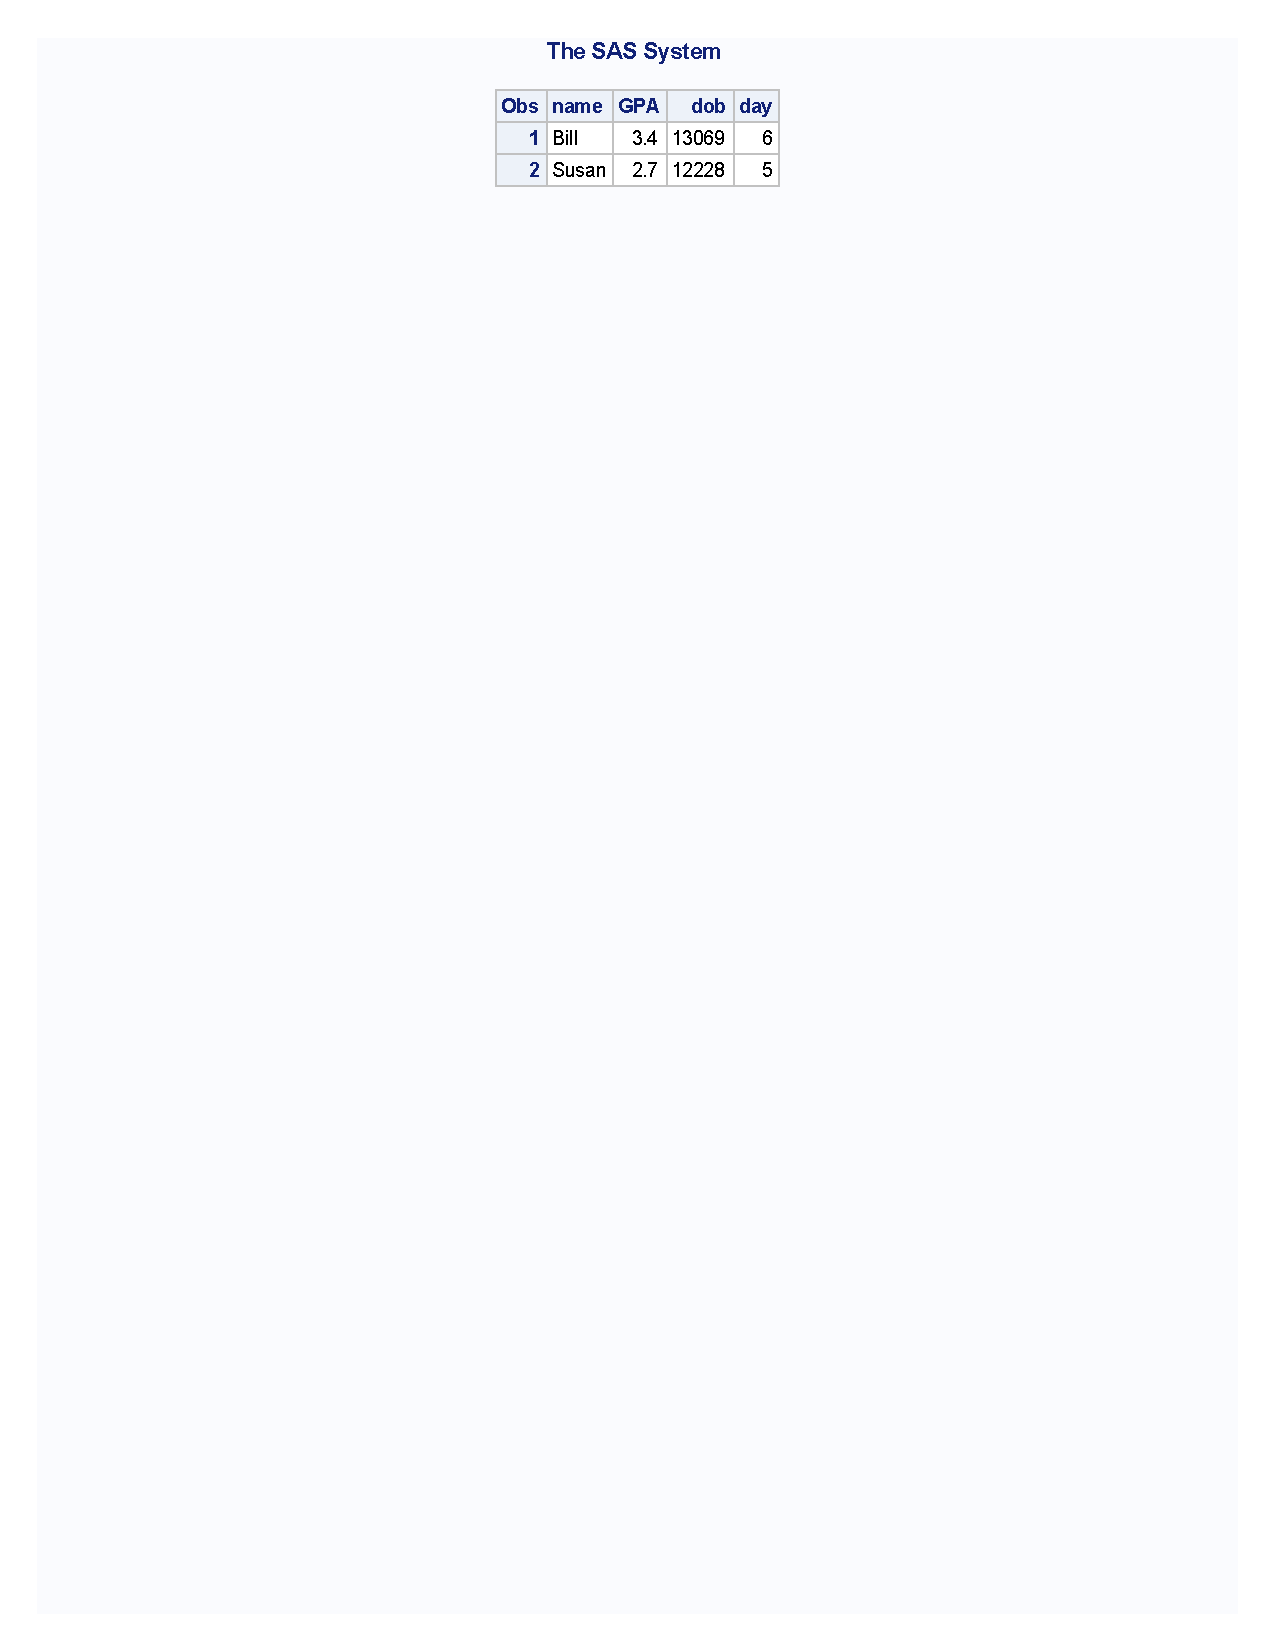
\includegraphics[trim=7.5cm 24.5cm 7.5cm 1.5cm,clip,width=1.0\textwidth]{L6_noformat.pdf}
\emp
\bmp{0.03\textwidth} \hspace{0.1in} \emp
\bmp{0.4\textwidth}
SAS stores dates as the number of days since January 1, 1960. \\
\vskip5pt
\begin{tabular}{lr}
-2 & Dec 30, 1959 \\
-1 & Dec 31, 1959 \\
 0 & Jan 1, 1960 \\
 1 & Jan 2, 1960 \\
 2 & Jan 3, 1960 \\
 7 & Jan 8, 1960 \\
\end{tabular}\\
\vskip5pt
\oyo What is the interpretation of 13069?
\emp
\end{frame}


\begin{frame}[fragile]
\ft{SAS days}
\bmp{0.60\textwidth}
\footnotesize
\begin{code}{.0}
DATA work.class;
  INPUT name \$ GPA dob MMDDYY10. ;
  day = WEEKDAY(dob);
  DATALINES ;
  Bill  3.4  10/13/1995
  Susan 2.7  6/24/1993
  ;
RUN ;
\end{code}
\vskip10pt
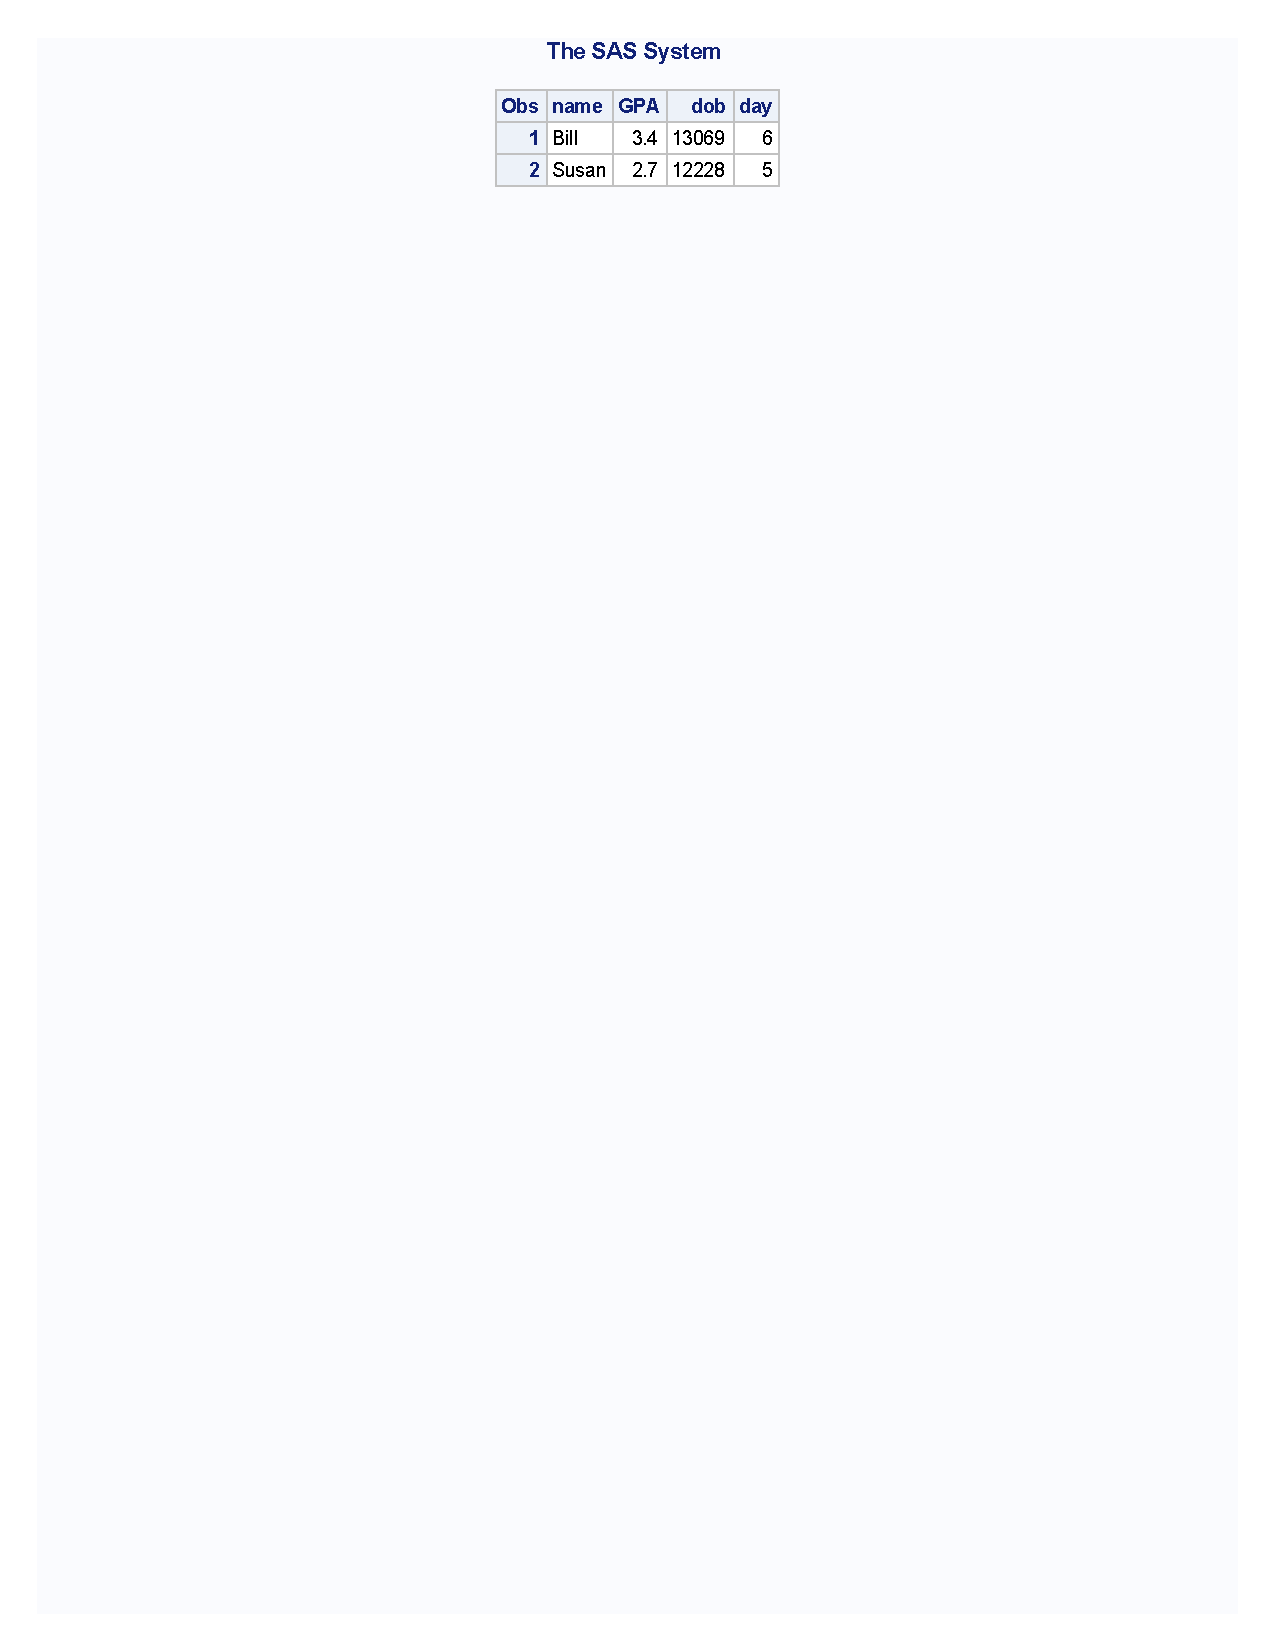
\includegraphics[trim=7.5cm 24.5cm 7.5cm 1.5cm,clip,width=1.0\textwidth]{L6_noformat.pdf}
\emp
\bmp{0.03\textwidth} \hspace{0.1in} \emp
\bmp{0.4\textwidth}
\oyo Examine the help file for the WEEKDAY informat.  What does a value of 6 mean?
\emp
%1 = Sunday
%2 = Monday
%3 = Tuesday
%4 = Wednesday
%5 = Thursday
%6 = Friday
%7 = Saturday
\end{frame}

\begin{frame}[fragile]
\ft{SAS formats (variable \emph{value} display)}
\hspace*{-0.3in}
\bmp{0.53\textwidth}
\footnotesize
\begin{code}{.0}
PROC PRINT DATA = work.class ;
   \textcolor{OrangeRed}{FORMAT dob DATE9.}
          \textcolor{OrangeRed}{day WEEKDATE9. ;}
RUN ;



\end{code}
\begin{itemize}
\item Formats applied in \ttt{PROCs} are temporary
\item Only applies for the duration of the procedure
\end{itemize}
\emp
\bmp{0.03\textwidth} \hspace{1in} \emp
\bmp{0.53\textwidth}
\footnotesize
\begin{code}{.0}
DATA work.class2 ;
   SET class;
   \textcolor{OrangeRed}{FORMAT dob DATE9.}
          \textcolor{OrangeRed}{day WEEKDATE9. ;}
RUN ;
PROC PRINT DATA = work.class2 ;
RUN ;
\end{code}
\begin{itemize}
\item Formats applied in \ttt{DATA} are permanent
\item Such formats will be applied to all procedures
\end{itemize}
\emp
\end{frame}

\begin{frame}[fragile]
\ft{SAS labels (variable \emph{name} display)}
\hspace*{-0.3in}
\bmp{0.70\textwidth}
\footnotesize
\begin{code}{.0}
PROC PRINT DATA = work.class \textcolor{OrangeRed}{LABEL} ;
   \textcolor{OrangeRed}{LABEL dob = "Date of Birth"}
         \textcolor{OrangeRed}{gpa = "Grade Point Average" ;}
RUN ;
\end{code}
%\vskip5pt
\footnotesize
\begin{code}{.0}
DATA work.class2 ;
   SET class ;
   \textcolor{OrangeRed}{LABEL dob = "Date of Birth"}
         \textcolor{OrangeRed}{gpa = "Grade Point Average" ;}
RUN ;
PROC PRINT DATA = work.class2 \textcolor{OrangeRed}{LABEL} ;
RUN ;
\end{code}
\emp
\bmp{0.35\textwidth}
\begin{itemize}
\item Labels applied in \ttt{PROCs} are temporary
\item Only applies for the duration of the procedure
\item[]
\item Labels applied in \ttt{DATA} are permanent
\item Such formats will be applied to all procedures
\item[]
\end{itemize}
\emp
\end{frame}

\begin{frame}[fragile]
\ft{Before and after}
\hspace*{-0.3in}
\bmp{0.65\textwidth}
\footnotesize
\begin{code}{.0}
PROC PRINT DATA = work.class ;
RUN ;
\end{code}

\begin{code}{.0}
PROC PRINT DATA = work.class LABEL ;
   FORMAT dob DATE9.
          day WEEKDATE9. ;
   LABEL dob = "Date of Birth"
         gpa = "Grade Point Average" ;
RUN ;
\end{code}
\emp
\bmp{0.03\textwidth} \hspace{1in} \emp
\bmp{0.45\textwidth}
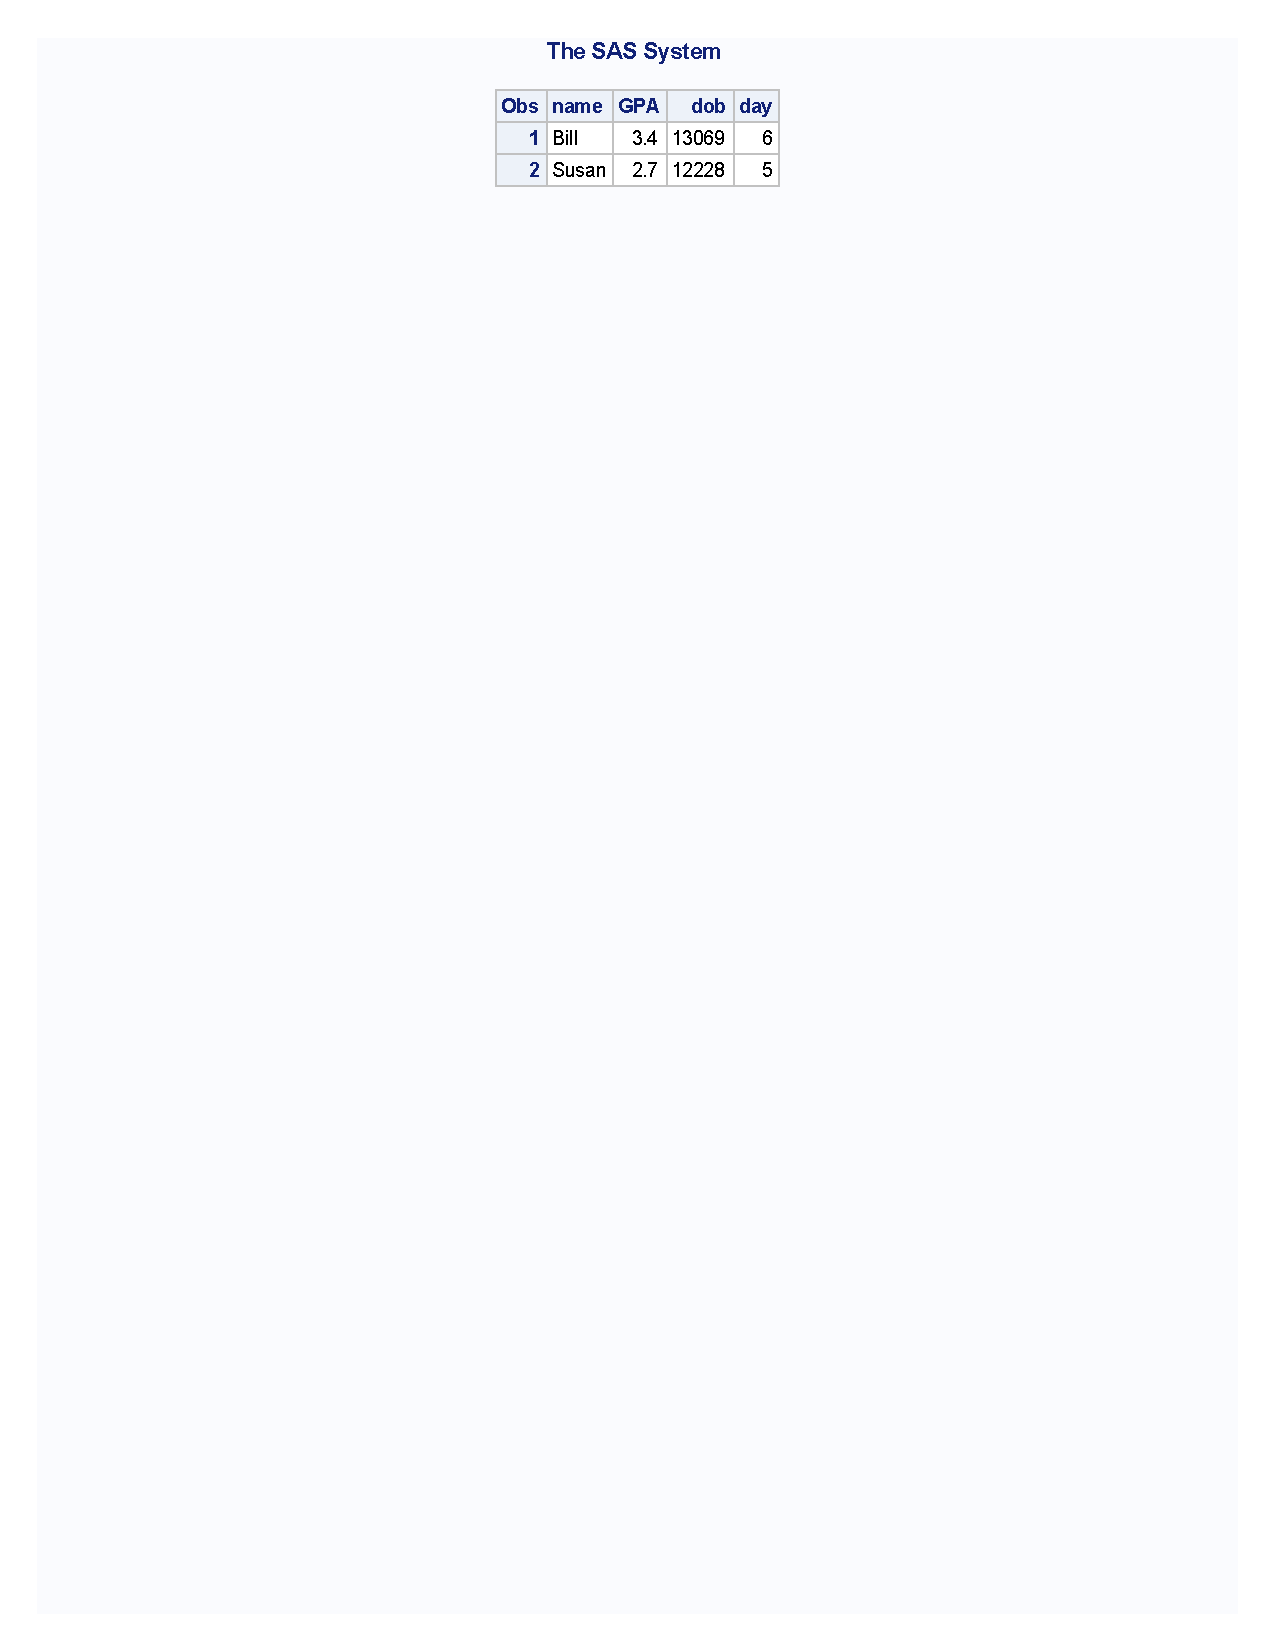
\includegraphics[trim=6.5cm 24.5cm 6.5cm 1.5cm,clip,width=1.0\textwidth]{L6_noformat.pdf}\\
\vskip30pt
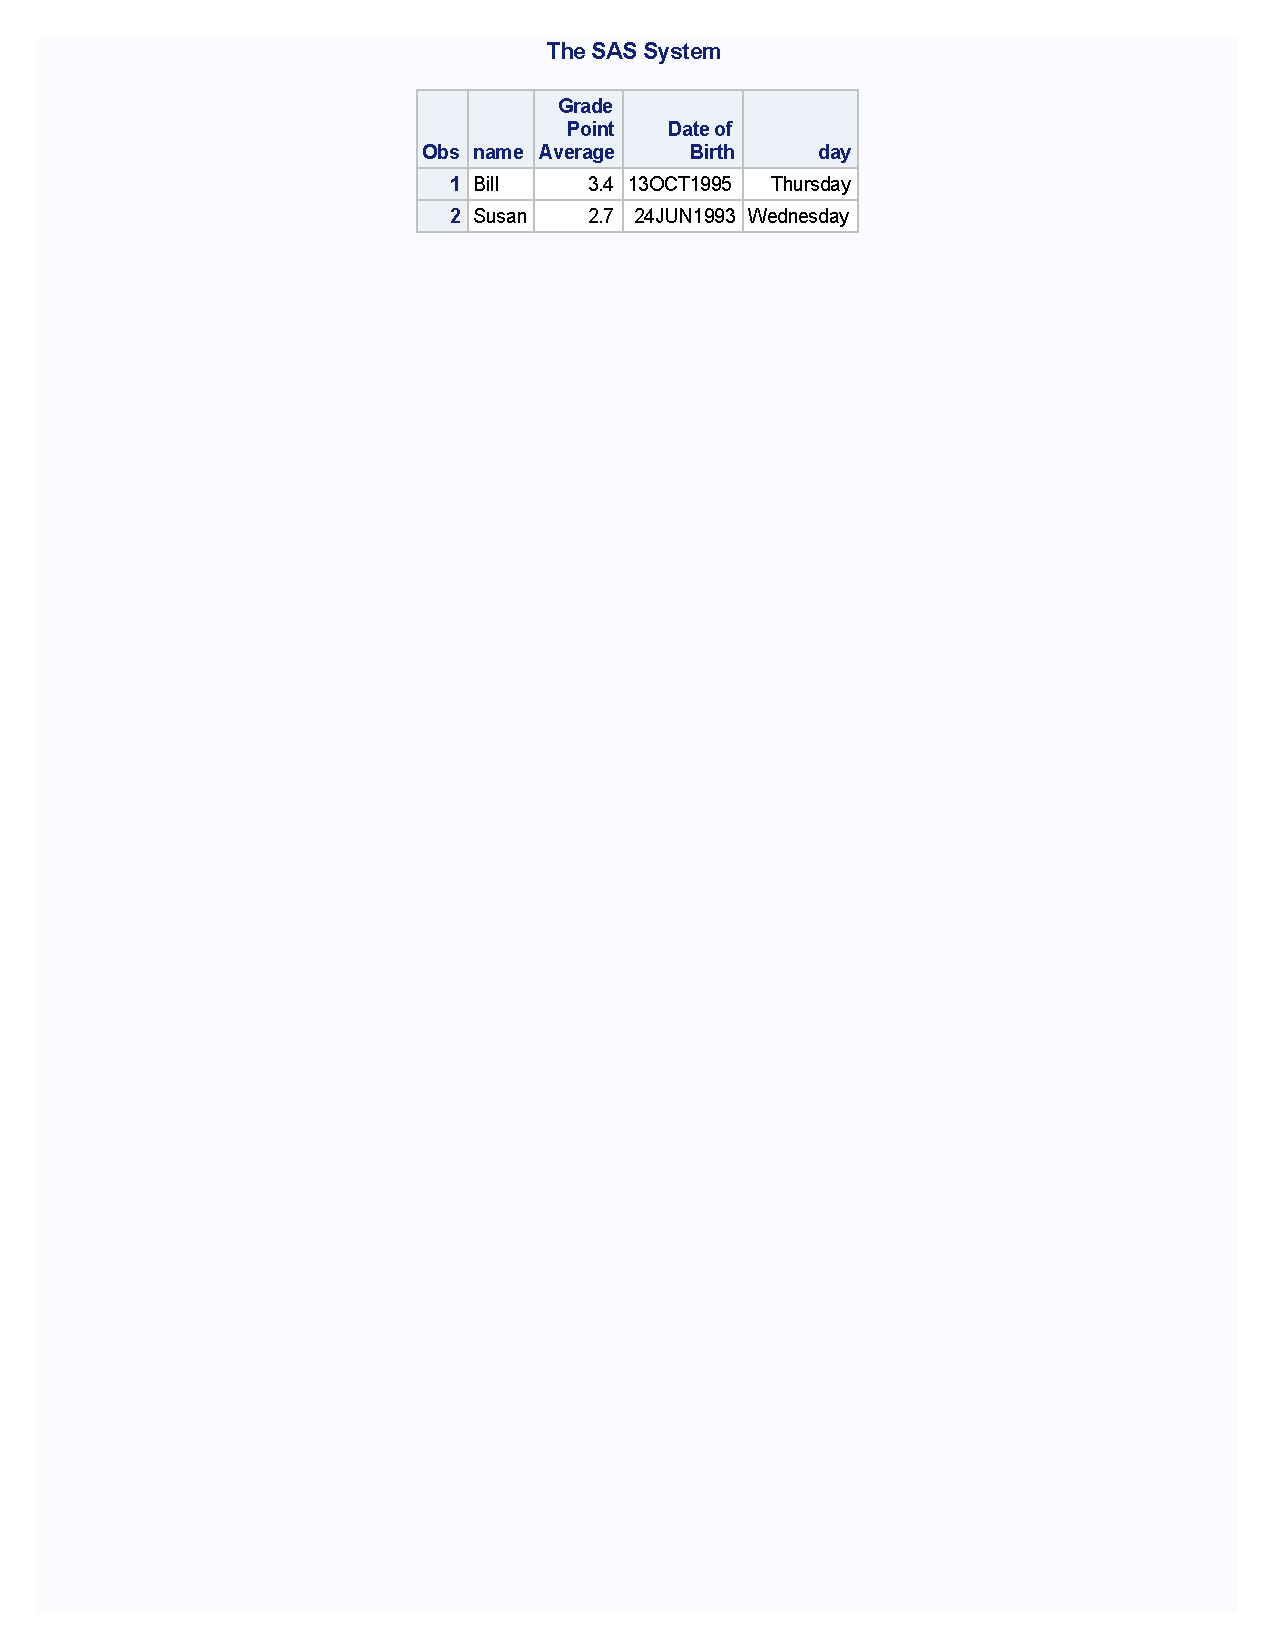
\includegraphics[trim=6.5cm 23.5cm 6.5cm 1.5cm,clip,width=1.0\textwidth]{L6_format.pdf}
\emp
\end{frame}

%===========================================================================================================================
\section[PROC FORMAT]{PROC FORMAT}
%===========================================================================================================================
\subsection{}
\begin{frame}
\tableofcontents[currentsection, hideallsubsections]
\end{frame}

\begin{frame}[fragile]
\ft{PROC FORMAT}
\ttt{DATE9., COMMA8.}, etc., are examples of formats built in to SAS.  You can create your own custom format for either character or numeric variables with \ttt{PROC FORMAT}.
\hspace{-0.3in}
\bmp{0.82\textwidth}
\footnotesize
\begin{code}{.0}
PROC FORMAT ;
   VALUE \textcolor{OrangeRed}{\emph{nameA}} \emph{range1} = "formatted value 1"
               \emph{range2} = "formatted value 2" ;

   VALUE \textcolor{OrangeRed}{\emph{\$nameB}} \emph{"range1"} = "formatted value 1"
                \emph{"range2"} = "formatted value 2" ;
RUN ;

PROC PRINT DATA = example ;
    FORMAT var1 \textcolor{OrangeRed}{nameA.} var2 \textcolor{OrangeRed}{\$nameB.} var3 \textcolor{OrangeRed}{nameA.} ;
RUN;
\end{code}
\emp
\bmp{0.25\textwidth}
\begin{itemize}
\item[]
\item \textcolor{OrangeRed}{\emph{nameA}} formats a numeric value
\item[]
\item \textcolor{OrangeRed}{\emph{\$nameB}} formats a character value
\end{itemize}
\emp
\end{frame}


\begin{frame}
\ft{PROC FORMAT - range key words}
{\renewcommand{\arraystretch}{1.3}
\begin{tabular}{r p{8.0cm}}
\hline
\textbf{Keyword} &  \textbf{Description} \\
\hline
hyphen ($-$) & continuous range \\
LOW/HIGH & used in ranges to indicate lowest/highest non-missing value \\
less than ($<$) & used in ranges to exclude end point \\
OTHER & assigns format to any values not yet listed \\
\hline
\end{tabular}}
\end{frame}


\begin{frame}
\ft{PROC FORMAT - ranges}
{\resizebox{1.0\textwidth}{!}
{\renewcommand{\arraystretch}{1.3}
\begin{tabular}{r p{3cm} p{5.0cm}}
\hline
\textbf{Value in} &  &  \\
\textbf{data set} & \textbf{Value display} & \textbf{Explanation} \\
\hline
``A'' = & ``Asia'' & A is a character value, goes in quotes\\
1,3,5 = & ``Odd''  & looking for numeric values 1 3 or 5\\
500-high = & ``Upper end'' & numeric values from 500 to infinity\\
3-$<$13 = & ``Child'' & numeric values between 3 and 13, excluding 13 exactly \\
OTHER = & ``anything else'' & any other value \\
\hline
\end{tabular}}}
\end{frame}




\begin{frame}[fragile]
\ft{\texttt{Babies.csv}}
\begin{tabular}{r|l}
\ttt{bwt} & baby's weight at birth in ounces\\
\ttt{parity} & 0=first born, 1=otherwise\\
\ttt{smoke} & smoking status of mother: 0=not now, 1=yes now\\
\end{tabular}
\vskip10pt
\bmp{1.0\textwidth}
\footnotesize
\begin{code}{.0}
PROC FORMAT ;
   VALUE birthorder 0 = "first born"
                    1 = "otherwise" ;

   VALUE smokestatus 0 = "not now"
                     1 = "yes now" ;

   VALUE birthweight low-88   = "under"
                     88<-high = "normal" ;
RUN ;
\end{code}
\emp
\end{frame}

\begin{frame}[fragile]
\ft{Two categorical variables, with and without formats}
\hspace*{-0.3in}
\bmp{0.55\textwidth}
\footnotesize
\begin{code}{.0}
PROC FREQ DATA = work.babies ;
   TABLES parity*smoke /
   NOROW NOCOL NOPERCENT ;
RUN;


\end{code}
\begin{center}
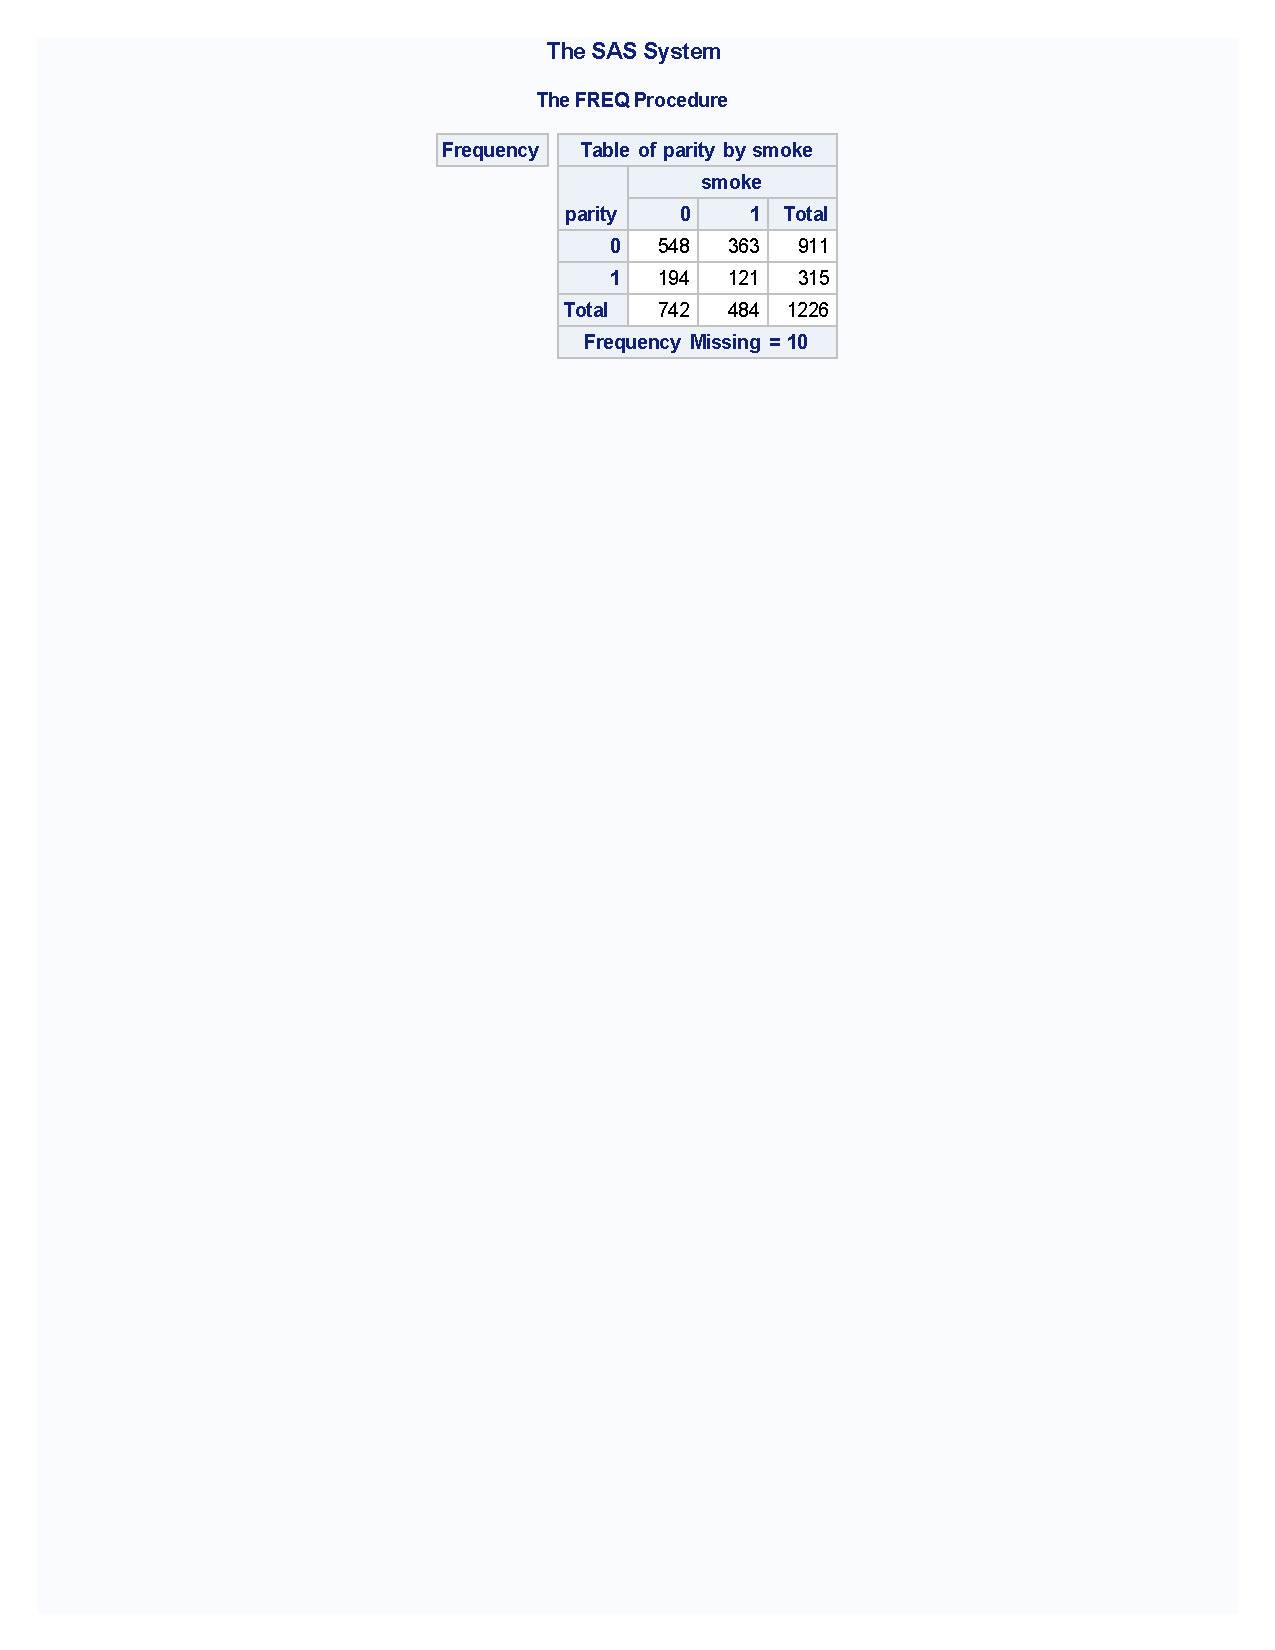
\includegraphics[trim=9.4cm 21.5cm 6.5cm 2.0cm,clip,width=0.72\textwidth]{L6_2waytableNOformat.pdf}
\end{center}
\emp
\bmp{0.03\textwidth} \hspace{1in} \emp
\bmp{0.55\textwidth}
\footnotesize
\begin{code}{.0}
PROC FREQ DATA = work.babies ;
    TABLES parity*smoke /
    NOROW NOCOL NOPERCENT ;
    \textcolor{OrangeRed}{FORMAT parity birthorder.}
           \textcolor{OrangeRed}{smoke smokestatus. ;}
RUN;
\end{code}
\begin{center}
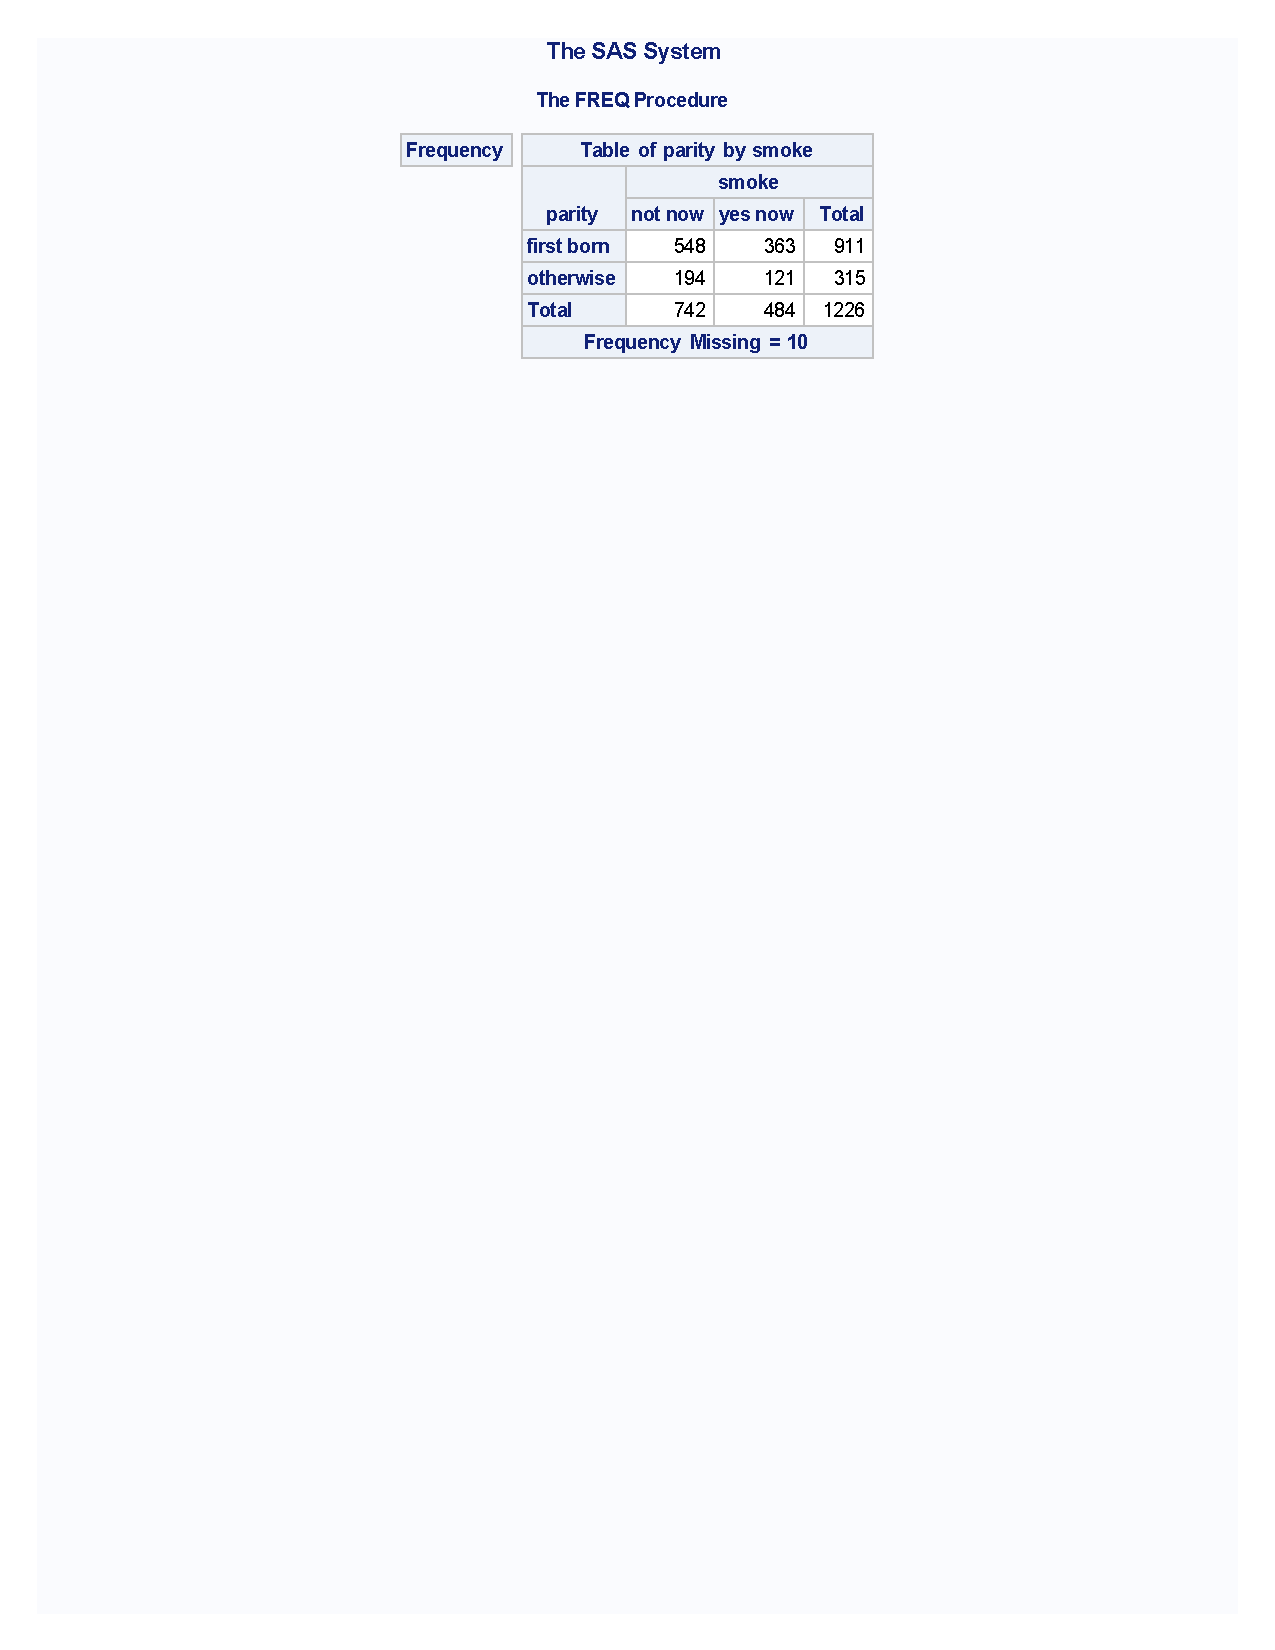
\includegraphics[trim=8.7cm 21.5cm 6.5cm 2.0cm,clip,width=0.8\textwidth]{L6_2waytableWITHformat.pdf}
\end{center}
\emp
\end{frame}

\begin{frame}[fragile]
\ft{One quantitative variable, with and without format}
\hspace*{-0.3in}
\bmp{0.55\textwidth}
\footnotesize
\begin{code}{.0}
PROC FREQ DATA = work.babies ;
   TABLES bwt ;
RUN;

\end{code}
\begin{center}
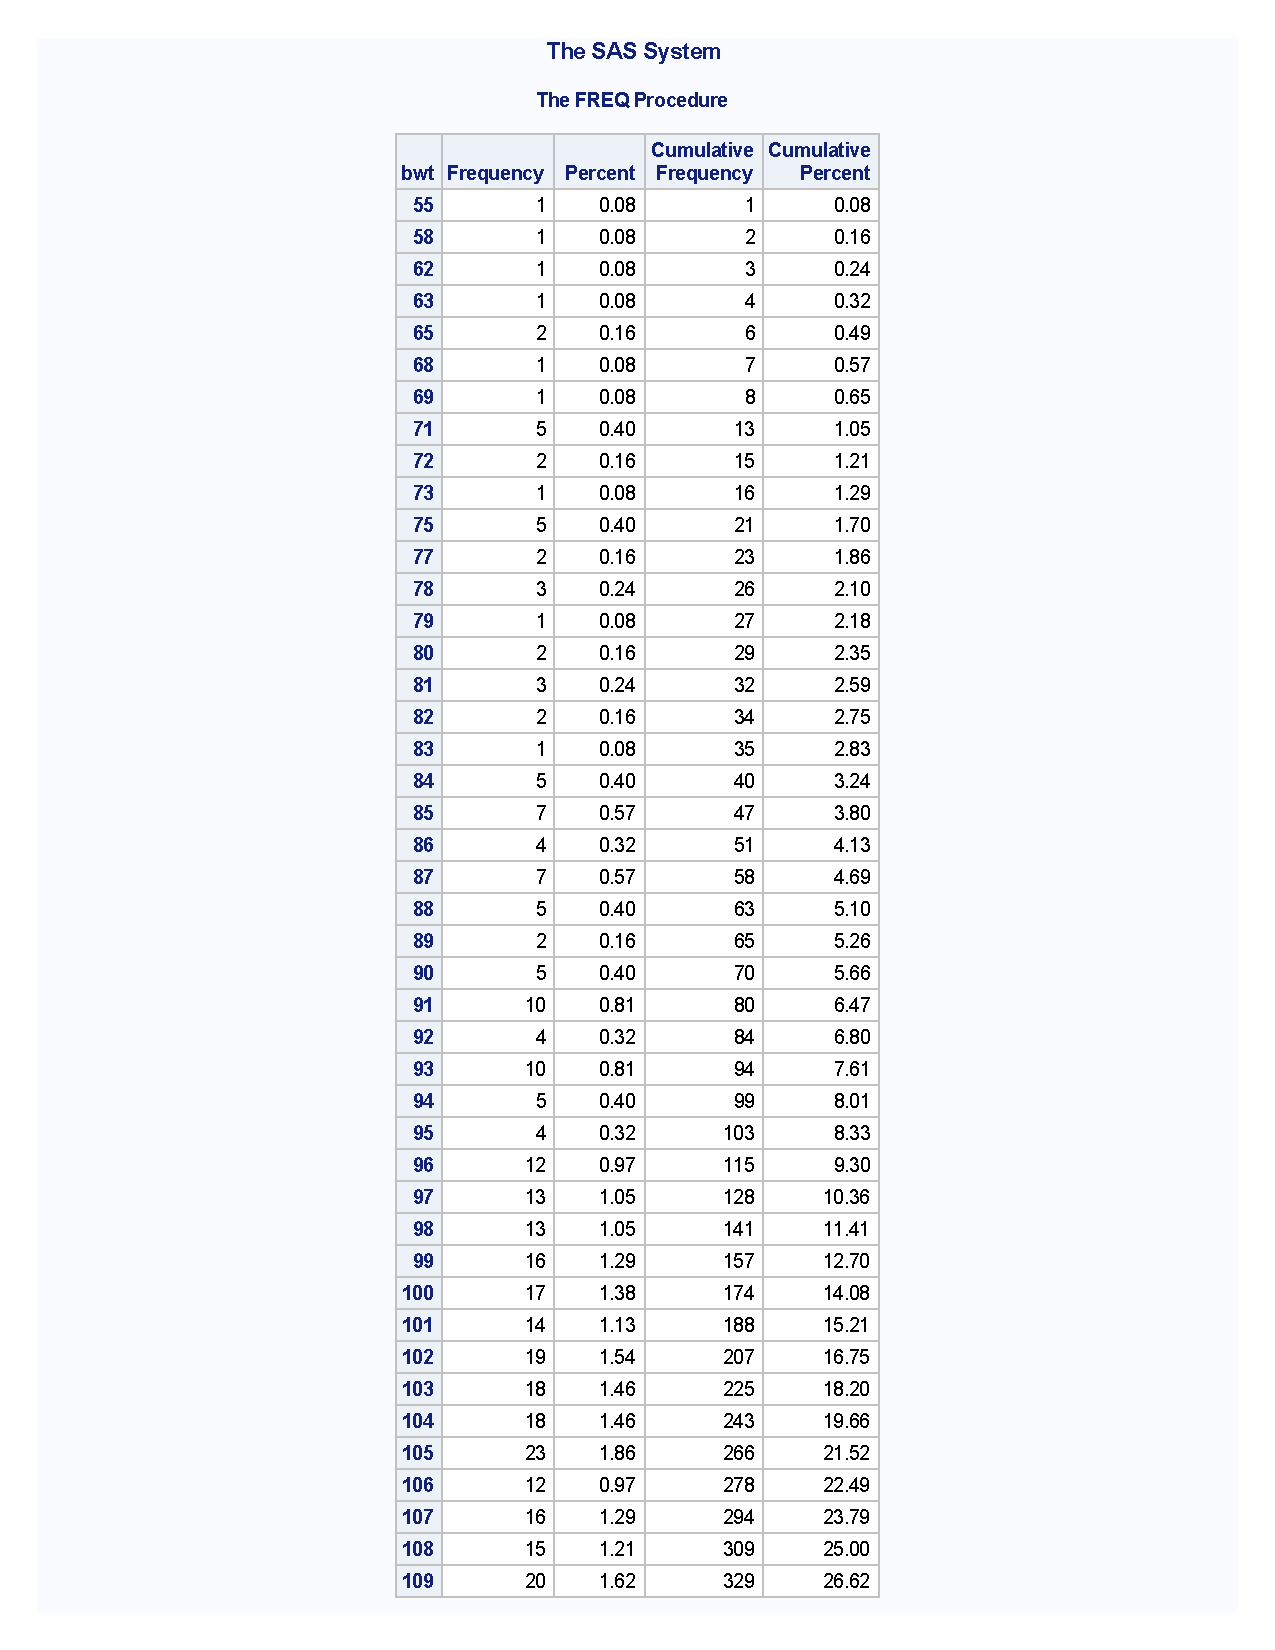
\includegraphics[trim=6cm 15cm 6.5cm 2.0cm,clip,width=0.72\textwidth]{L6_1waytableNOformat.pdf}
\end{center}
\emp
\bmp{0.03\textwidth} \hspace{1in} \emp
\bmp{0.55\textwidth}
\footnotesize
\begin{code}{.0}
PROC FREQ DATA = work.babies ;
    TABLES bwt ;
    \textcolor{OrangeRed}{FORMAT bwt birthweight. ;}
RUN;
\end{code}
\begin{center}
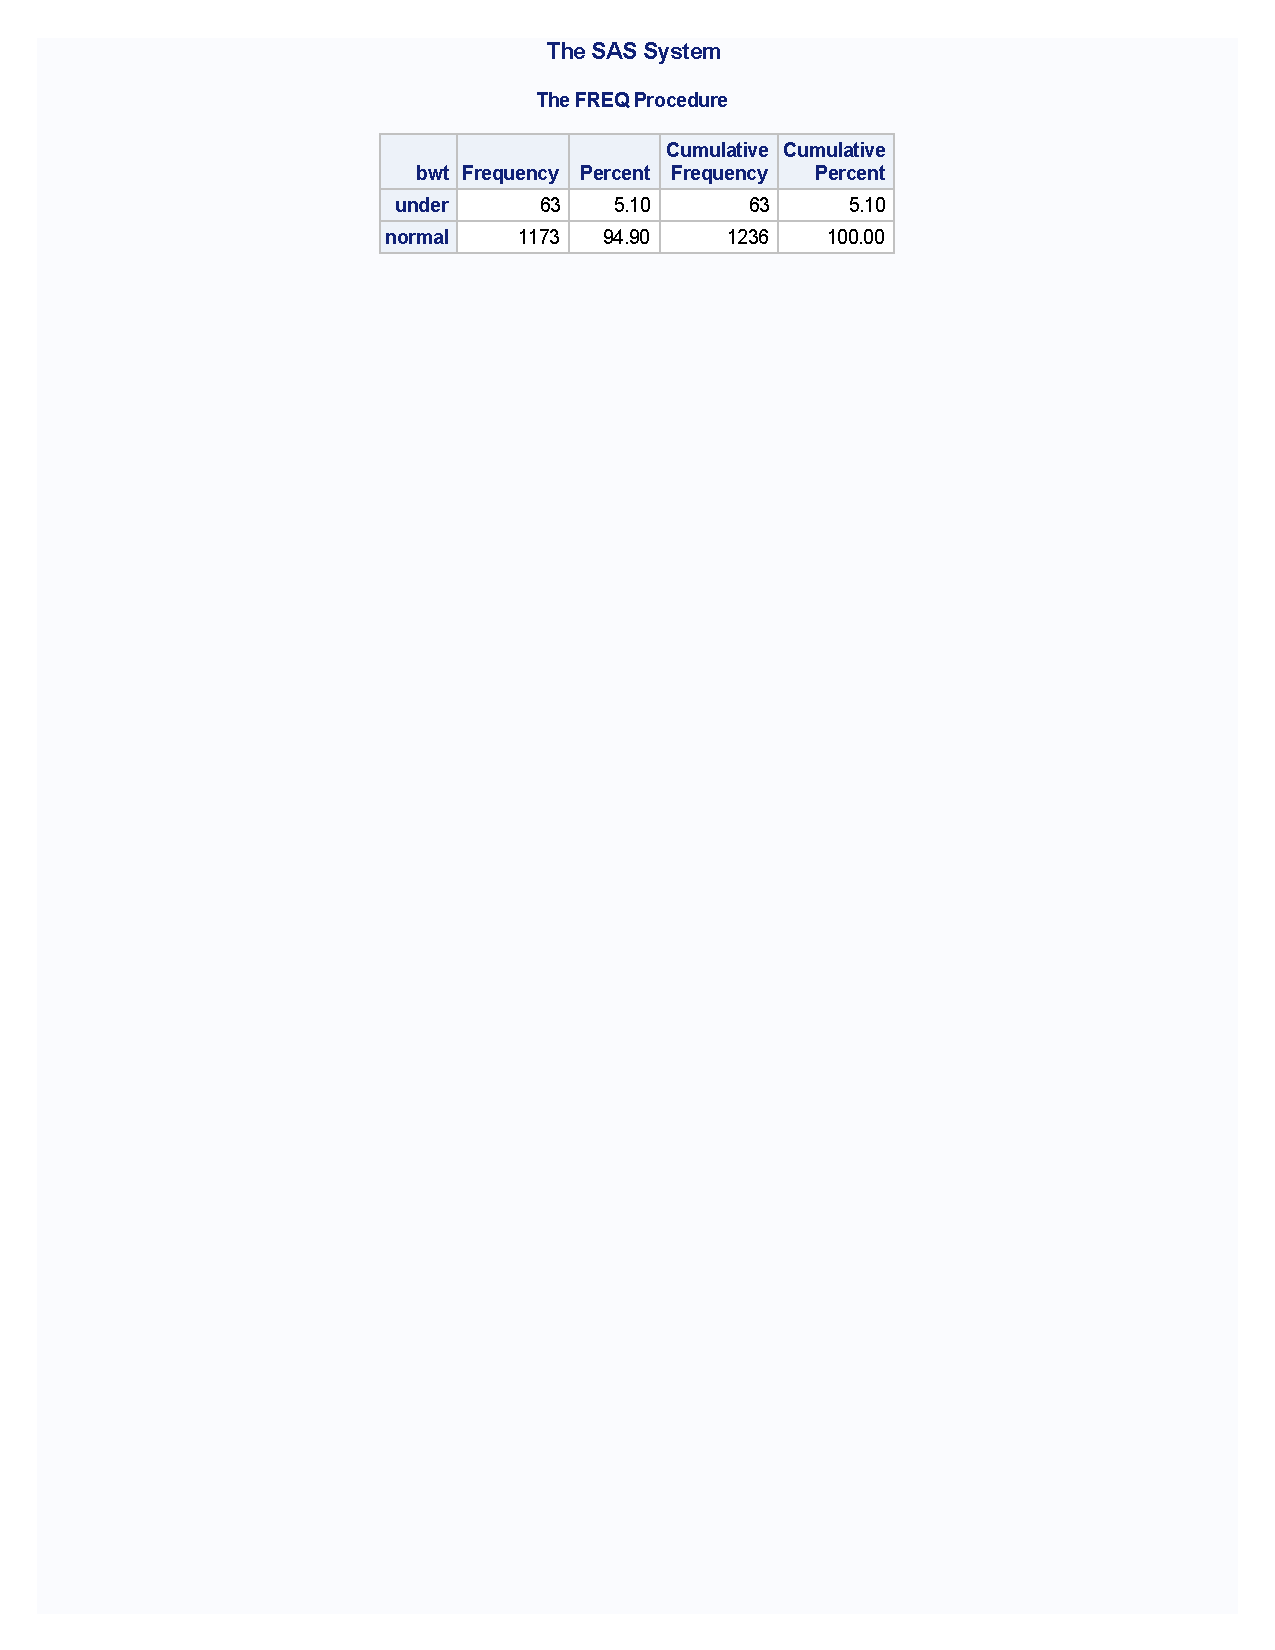
\includegraphics[trim=6.0cm 15.5cm 6.0cm 2.0cm,clip,width=0.8\textwidth]{L6_1waytableWITHformat.pdf}
\end{center}
\emp
\end{frame}

\end{document} 